\newpage

\begin{problem}
  Find the best minimax approximation from the space of polynomials of
  degree at most one to $f (x) = x^2 \, , x \in [0, 1]$. Plot the result
  together with the original function. Plot the error function.
\end{problem}

\begin{solution}
  Theorem 7.4 gives us that if we find a function with 3 points in the
  interval where the error equals the maximum error then we have our
  best approximation. From figure~\ref{fig:2:error} it is clear that
  the function $x - 1/8$ in figure~\ref{fig:2:approx} that was found
  in an earlier homework satisfies the criteria of theorem 7.4 and is
  this a best approximation.
  
  \begin{figure}[ht!]
    \centering 
    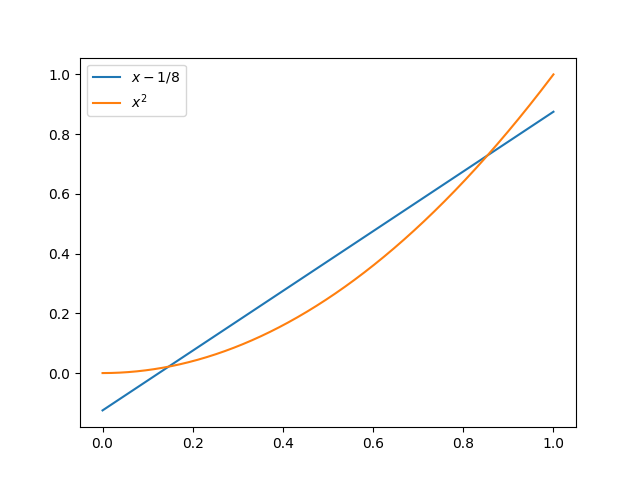
\includegraphics[scale = 0.5]{code/task_2_approximation.png}
    \caption{$x - 1/8$ and $x^2$}
    \label{fig:2:approx}
  \end{figure}

  \begin{figure}[ht!]
    \centering 
    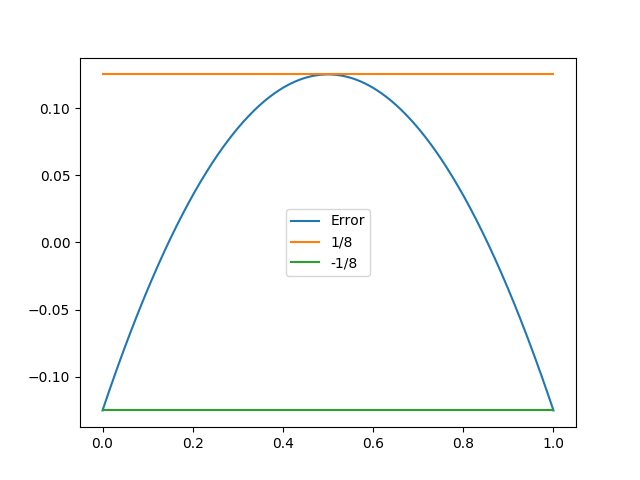
\includegraphics[scale = 0.5]{code/task_2_error.png}
    \caption{$x - 1/8 - x^2$}
    \label{fig:2:error}
  \end{figure}

\end{solution}

%%% Local Variables:
%%% mode: latex
%%% TeX-master: "report"
%%% End:
